% @Author: AnthonyKenny98
% @Date:   2019-11-02 19:23:52
% @Last Modified by:   AnthonyKenny98
% @Last Modified time: 2019-11-03 00:28:50

To restate, the aim of this thesis is to design a computer processor with reduced execution time of motion planning algorithms, such as \ac{RRT}. As such, it is important to understand the elements of the algorithm that have the highest percentage of CPU execution time. To determine this, it was necessary to implement my own, naive but typical, \ac{RRT} in C. This program could then be compiled and analysed using a software performance profiling tool. With this, I could design experiments to determine the critical RRT functions (those occupying a majority of CPU time) and see how this varies given different paramaters.

\subsubsection{Implementation of Algorithm}
The first step was to source a simple, naive implementation of RRT in C that could be analysed. The two options were to either find an existing, public implementation or to develop my own. Many implementations I found online\cite{RoboJackets2019}\cite{Planning2019}\cite{Sourishg2017}\cite{Vss2sn2019} were unsuitable for my purposes, as they had extraneous \ac{GUI}s, reliance on external \ac{API}s, and other features that distorted analysis of algorithmic hotspots. This made them largely useless for my performance analysis. I needed a clean, minimal implementation of RRT so that I could easily identify the percentage of CPU time each function took up.  \\ 

As such, I implemented my own version. It can be found \href{https://github.com/AnthonyKenny98/Thesis/tree/master/my_rrt}{here}. It follows the Algorithm defined above closely. I took care to be able to parametrize factors such as Number of Nodes, Number of Obstacles, Obstacle Size, State Space Size, and Epsilon (acceptable distance between two nodes). For monitoring correctness, I build in an optional \ac{GUI} that shows the tree, starting node, and obstacles. Figure \ref{table:rrtGui} demonstrates the \ac{GUI} and the \ac{RRT} implementation.

\begin{figure}[H]
\begin{center}
\begin{tabular}{c  c}
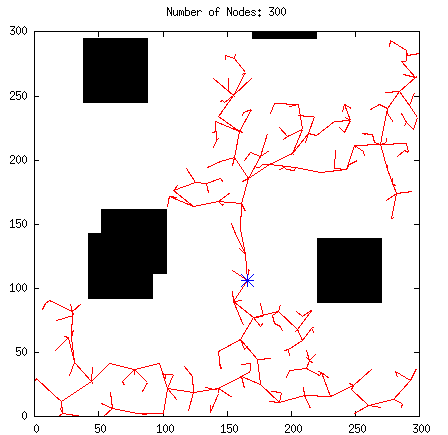
\includegraphics[width=0.5\linewidth]{../master/rrt/img/sampleRRT1.png} & 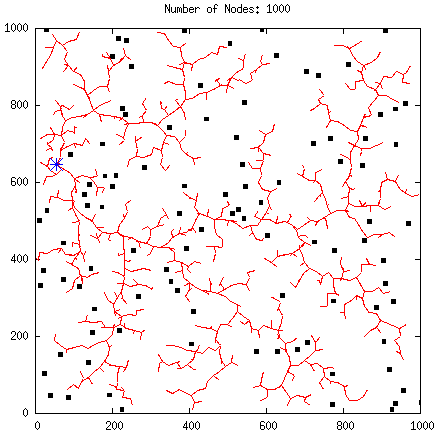
\includegraphics[width=0.5\linewidth]{../master/rrt/img/sampleRRT2.png} \\
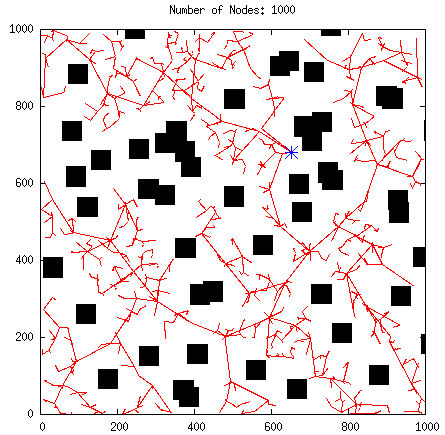
\includegraphics[width=0.5\linewidth]{../master/rrt/img/sampleRRT3.png} & 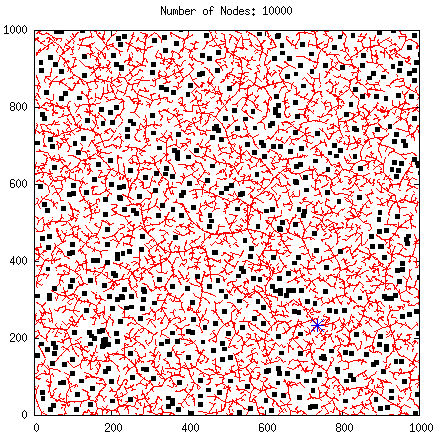
\includegraphics[width=0.5\linewidth]{../master/rrt/img/sampleRRT4.png}
\end{tabular}
\caption{RRT Implementation shown by \ac{GUI}}
\label{table:rrtGui}
\end{center}
\end{figure}

\subsubsection{Top Down Analysis}{}

The idea of top-down analysis is a practical method to quickly identify true bottlenecks in out-of-order processors, explained well in the paper by A. Yasin\cite{Yasin2014}. It was influenced by a basic approach that examines the functions that take the highest percentage of CPU time, and drills down to examine their sub-routines. This functionality is provided by software by Intel, called VTune Amplifier. \\

VTune Amplifier performance profiler is an application for software performance analysis. It provides functionality to examine hotspots for CPU execution time through a top down analysis, shown below in Figure \ref{fig:topdown}. As can be seen from the figure, the top down analysis tool shows the percentage of CPU time taken up by each function. I used this tool to profile the algorithm's performance as I changed certain parameters.

\begin{figure}[H]
\begin{center}
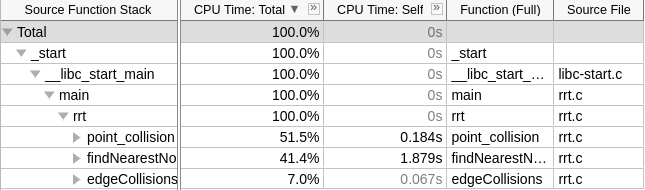
\includegraphics[width=0.8\linewidth]{../master/rrt/img/topDownAnalysis.png}
\caption{Top Down Analysis Functionality provided by VTune Amplifier}
\label{fig:topdown}
\end{center}
\end{figure}


\subsubsection{Experimental Design}

As stated above, I parametrized my implementation to be able to vary state space, number of nodes, number of obstacles, obstacle size, and  Epsilon. When considering the application of autonomous drones, the two most important factors are number of nodes and number of obstacles. Number of nodes is important for any implementation of RRT, as this is a determining factor of execution speed. A higher number of nodes will also yield shorter paths/higher probability of finding a path to a goal. Number of obstacles is important for autonomous drones, as the obstacles they face in their operating environments (complex natural environments) are often irregularly shaped. As such, these obstacles must often be discretized into a number of smaller obstacles. This is unlike applications such as robotic arms, where the size of (often regularly shaped) obstacles is more important. Given this, I ran a series of tests, varying number of nodes and number of obstacles, to determine the relative use of CPU time for each sub-routine in my RRT implementation.

\newpage

\subsubsection{Results}
The left side of Figure \ref{table:rrtPerformance} shows \% of CPU use for a given number of nodes, while the right side shows the same but for a given number of obstacles. the results below show that the three main sub-functions within the \ac{RRT} implementation are \texttt{edgeCollision()}, \texttt{pointCollision()}, and \texttt{findNearestNode()}. The importance of this is discussed in the design section.
\begin{figure}[H]
\begin{center}
\begin{tabular}{c | c}
Given \# of Nodes                                           & Given \# of Obstacles \\  
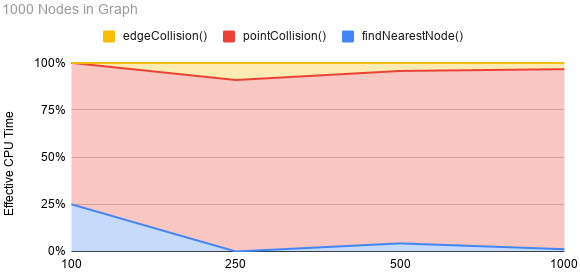
\includegraphics[width=0.45\linewidth]{../master/rrt/img/performance/nodes/1000nodes.png} & 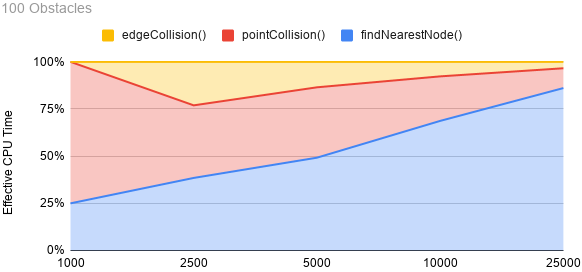
\includegraphics[width=0.45\linewidth]{../master/rrt/img/performance/obs/100obs.png} \\
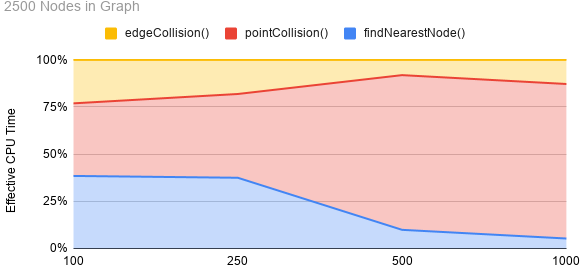
\includegraphics[width=0.45\linewidth]{../master/rrt/img/performance/nodes/2500nodes.png} & 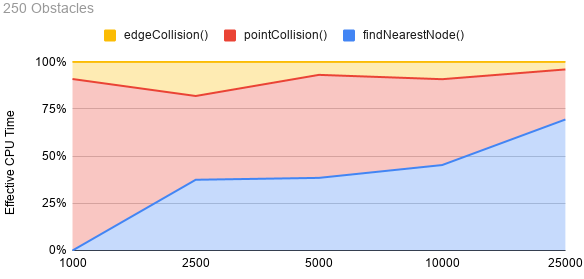
\includegraphics[width=0.45\linewidth]{../master/rrt/img/performance/obs/250obs.png} \\
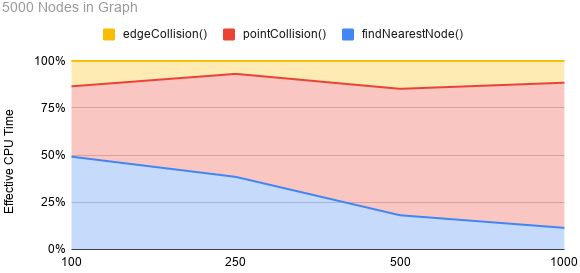
\includegraphics[width=0.45\linewidth]{../master/rrt/img/performance/nodes/5000nodes.png} & 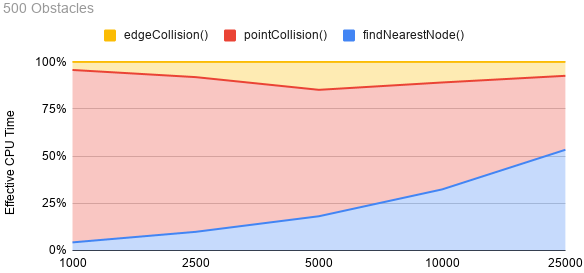
\includegraphics[width=0.45\linewidth]{../master/rrt/img/performance/obs/500obs.png} \\
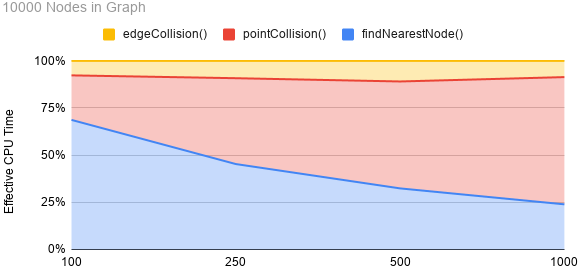
\includegraphics[width=0.45\linewidth]{../master/rrt/img/performance/nodes/10000nodes.png} & 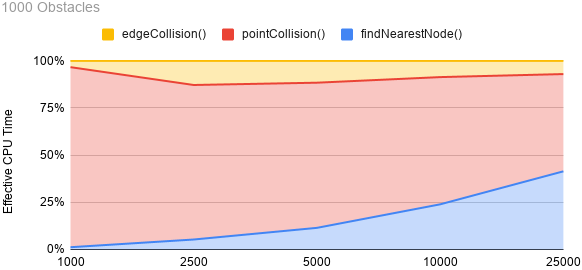
\includegraphics[width=0.45\linewidth]{../master/rrt/img/performance/obs/1000obs.png} \\
\end{tabular}
\caption{\% of CPU Time per Function}
\label{table:rrtPerformance}
\end{center}
\end{figure}

